% !TeX spellcheck = cs_CZ
%{\tikzset{external/prefix={tikz/FYZI/}}
% \tikzset{external/figure name/.add={ch46_}{}}
%=========================== Kapitola: Rohatka se západkou ========================================
\setchaptertoc
\chapter{Rohatka se západkou}\label{fyz:IchapXLVI}

  \section{Jak pracuje rohatka}\label{fyz:IchapXLVIsecI}
  \section{Rohatka jako stroj}\label{fyz:IchapXLVIsecII}
  \section{Vratnost v mechanice}\label{fyz:IchapXLVIsecIII}
  \section{Nevratnost}\label{fyz:IchapXLVIsecIV}
  \section{Uspořádání a entropie}\label{fyz:IchapXLVIsecV}
  \section{Příklady a cvičení}\label{fyz:IchapXLVIsecVI}

    \begin{figure}[ht!] %\ref{fyz:fig461}
      \centering
      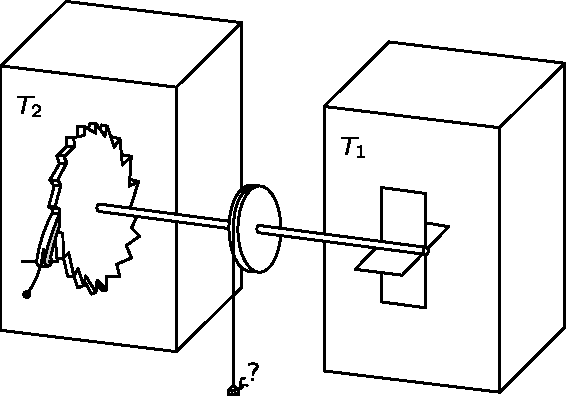
\includegraphics[width=0.7\linewidth]{fyz_fig461.pdf}
      \caption{ 
               (\cite[s.~707]{Feynman01})}
      \label{fyz:fig461}
    \end{figure}

    \begin{figure}[ht!] %\ref{fyz:fig462}
      \centering
      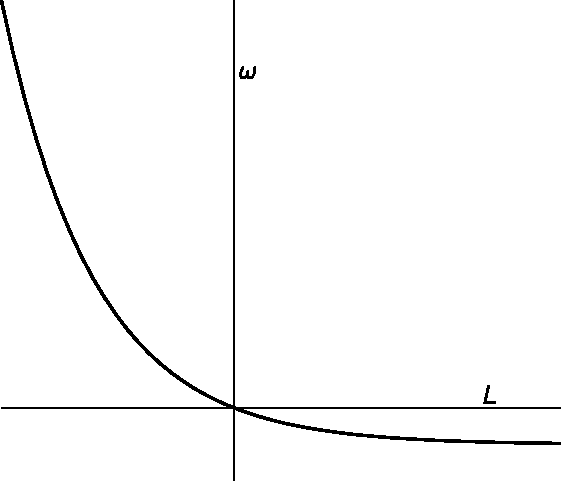
\includegraphics[width=0.7\linewidth]{fyz_fig462.pdf}
      \caption{ 
               (\cite[s.~707]{Feynman01})}
      \label{fyz:fig462}
    \end{figure}
    \todo[inline]{Kapitola fey1ch46 je zcela prázdná, pouze obrázky}     
%} %tikzset
%---------------------------------------------------------------------------------------------------